\section{Udvælgelse af gestik-par til pause og start}
\label{TestresultaterPauseStart}
%
Udvælgelsen af hvilket gestik-par, der skal knyttes til pause og start foretages på baggrund af testpersonernes begrundelser for til- og fravalg af de foreslåede gestikker. Der fokuseres først på hvilke gestik-par testpersonerne har inddraget i deres top tre rangering og i den forbindelse, om det er muligt at ekskludere nogle gestik-par. Derefter fokuseres der på testpersonernes begrundelser for, hvorfor de har valgt de gestik-par, som de har, hvorunder forbedringsforslag inkluderes, hvis testpersonerne fremsætter nogle. Afsnittet vil afslutningsvist ende ud i hvilket gestik-par, der vælges til at pause og starte musikken.\blankline
%
Få at få et overblik over, hvor ofte de syv forskellige gestik-par individuelt indgår på enten en første, anden eller tredje plads i top tre rangeringen opstilles følgende \autoref{fig:SamletTopTrePause}. 
%
\begin{figure}[H]
	\centering
	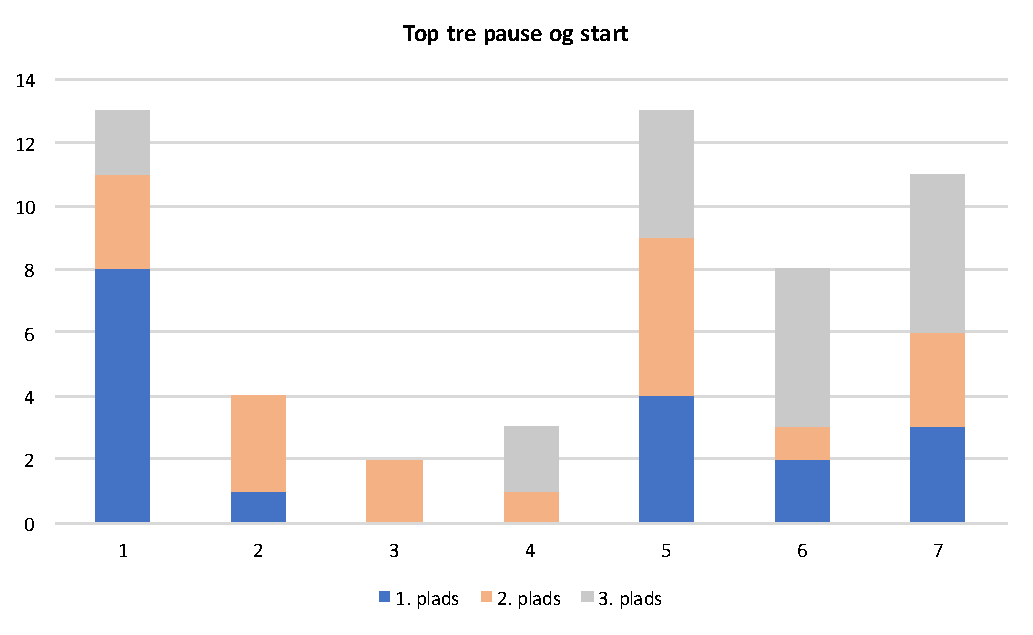
\includegraphics[resolution=300,width=0.9\textwidth]{Test1/DatabehandlingGrafer/TopTrePause}
	\caption{Søjlediagram over hvordan hvert gestik-par indgår i testpersonernes top tre i forhold til pause og start. Data forefindes i \autoref{app:TopTreRangeringPauseStart}.}
	\label{fig:SamletTopTrePause}
\end{figure}
\noindent
% 
På \autoref{fig:SamletTopTrePause} fremgår det tydeligt, at GP1, GP5, GP6 samt GP7 er de tre gestik-par, som uafhængigt af den specifikke plads, indgår flest gange i testpersonernes top tre. Derudover tyder det på, at hverken GP2, GP3 eller GP4 er specielt eftertragtet, da de henholdvis kun indgår fire, to og tre gange i testpersonernes samlede top tre, jævnfør \autoref{fig:SamletTopTrePause}. For at vurdere om der er belæg for, at ekskludere et eller flere gestik-par opstilles følgende \autoref{fig:DaarligstGestikPause}.  
%
\begin{figure}[H]
	\centering
	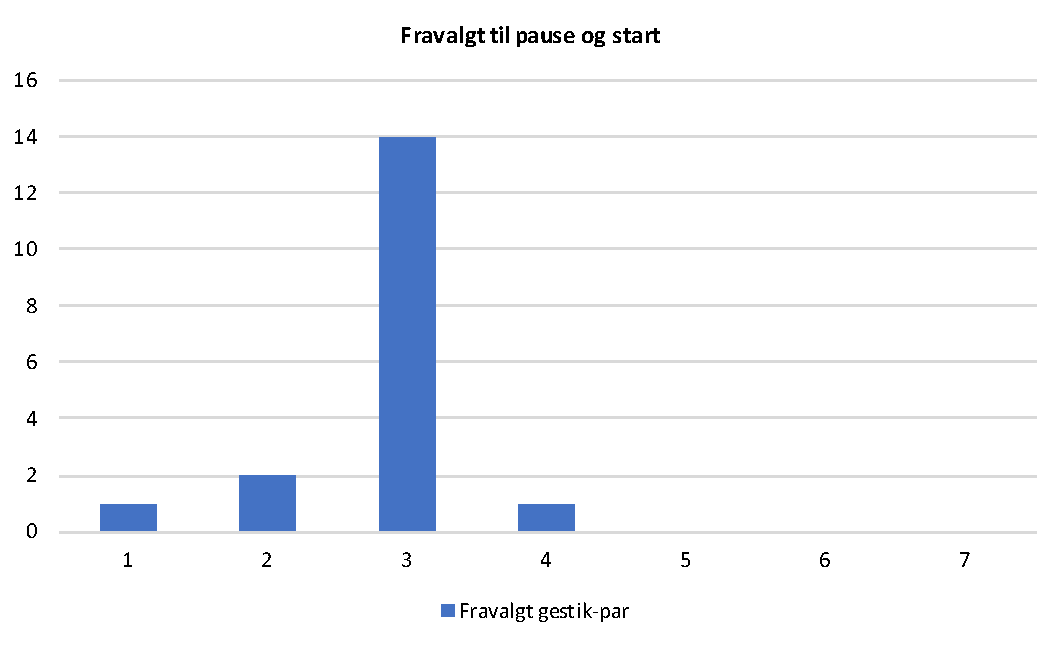
\includegraphics[resolution=300,width=0.9\textwidth]{Test1/DatabehandlingGrafer/FravalgtPause}
	\caption{Søjlediagram over hvilke gestik-par testpersonerne fravælger i forbindelse med pause og start.}
	\label{fig:DaarligstGestikPause}
\end{figure}
\noindent
%
På \autoref{fig:DaarligstGestikPause} opsummeres antallet af gange hvert gestik-par fravælges af testpersonerne. Da 14 ud af 18 testpersoner har fravalgt GP3 konkluderes det, at testpersonerne ikke bryder sig om GP3, hvorfor GP3 ekskluderes. På \autoref{fig:SamletTopTrePause} fremgår det, at GP4 aldrig tildeles en førsteplads og derudover kun indgår én og to gange på henholdvis en anden- og tredjeplads og selvom GP4 kun fravælges af en enkelt testperson, så vurderes det, at GP4 er overflødig og irrelevant. Der er derfor belæg for at ekskludere GP4. Tilsvarende er gældende for GP2, som kun indgår fire gange i testpersonernes samlede top tre og kun én gang tildeles en førsteplads, jævnfør \autoref{fig:SamletTopTrePause}, og derudover fravælges to gange, jævnfør \autoref{fig:DaarligstGestikPause}. I \autoref{app:TestresultaterPauseDaarlig} forefindes en dybere analyse af hvorfor testpersonerne fravælge de gestik-par, som de gør.

Ekskluderingen af de tre gestik-par medfører, at den efterfølgende analyse vil omhandle testpersonernes begrundelser for at vælge GP1, GP5, GP6 samt GP7.
%
\subsection{Testpersonernes begrundelse for valg af gestik-par 1}
\label{TestresultaterValgAfGestikkerBegrundelseGP1}
%
Med udgangspunkt i \autoref{fig:SamletTopTrePause} tildeles GP1 en førsteplads af otte testpersoner, en andenplads af tre testpersoner og en tredjeplads af to testpersoner. GP1 illustreres på \autoref{fig:GestikPar1Pause}. De testpersoner, som har tildelt GP1 en førsteplads, begrunder det ud fra en kombination af følgende egenskaber: 
%
\begin{multicols}{3}
    \begin{itemize}
        \item Simpel
        \item Enkel
        \item Logisk
        \item Naturlig
        \item Oplagt
        \item Nem at huske
        \item Nem at udføre
        \item Hurtig at udføre
        \item Giver mening
\end{itemize}
\end{multicols}
\noindent
%
Baseret på responsen fra TP3 og TP10 så er de, de eneste to testpersoner, som ikke er i tvivl om, at GP1 skal tildeles en førsteplads. TP3 benytter udelukkelsesmetoden til at argumentere for sin top tre og nævner i den forbindelse, at GP5, GP6 samt GP7 i højere grad minder om en mute-funktion fremfor pause- og startfunktion. At forbinde de tre gestik-par med en mute-funktion giver ikke mening i denne sammenhæng, da det er ret usandsynligt at musikken mutes fremfor at pauses, men i dette tilfælde danner det grundlag for TP3's top tre rangering. TP10 danner sin top tre rangering ud fra hvilke gestik-par, der er lavest risiko for at gengive anderledes og samtidig er det ikke en bevægelse, som testpersonen hyppigt laver. Dog pointerer TP5, at netop GP1 naturligt kan forekomme i ens kropssprog.
%
\begin{figure}[H]
	\centering
	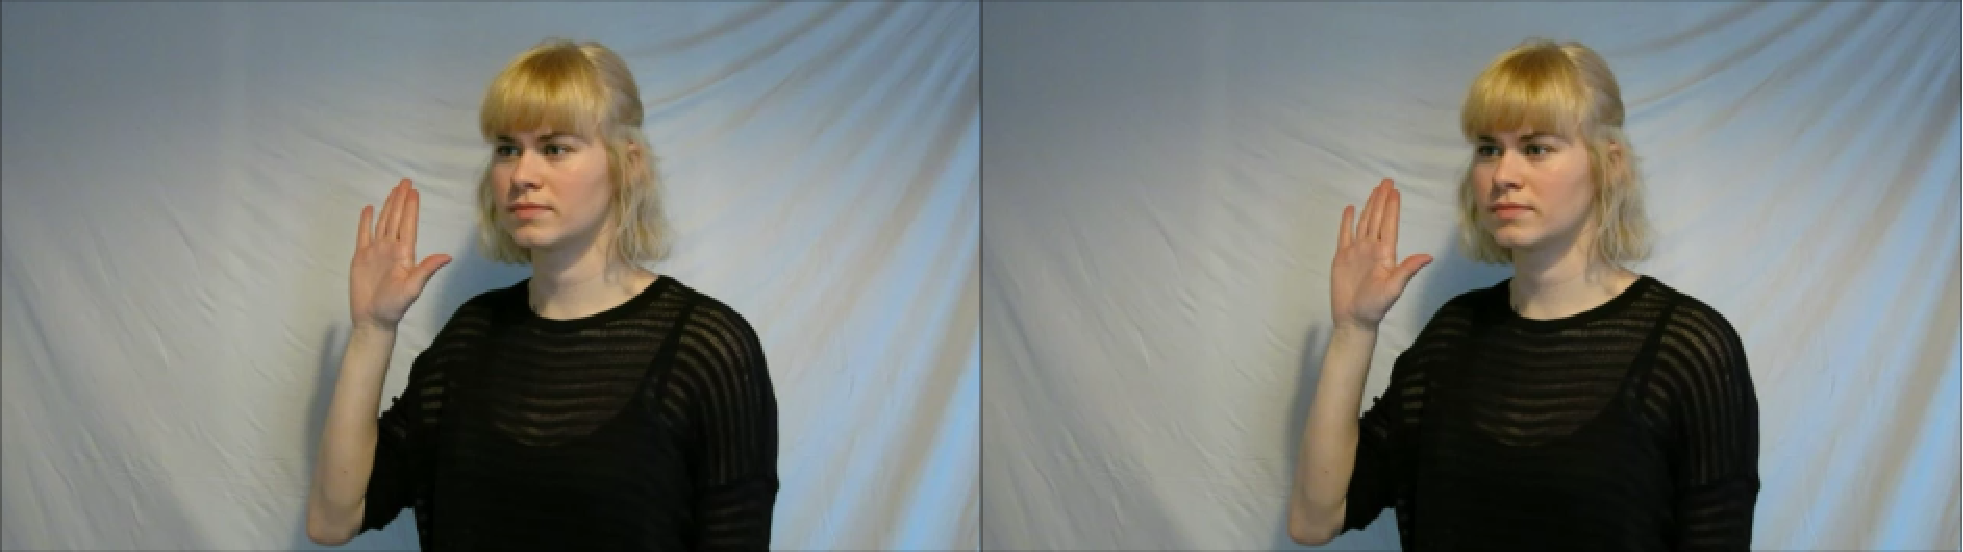
\includegraphics[resolution=300,width=0.9\textwidth]{Test1/Gestik-par/Gestik1_Pause}
	\caption{Illustration af gestik-par 1; stop-tegn til henholdsvis pause og start.}
	\label{fig:GestikPar1Pause}
\end{figure}
\noindent
%
De seks andre testpersoner, som har rangeret GP1 på en førsteplads, har alle tildelt GP5 enten en anden- eller tredjeplads. TP1 alternere mellem at have GP1 og GP5 på en førsteplads, hvorfor det ikke er endegyldigt at fastslå hvilket gestik-par TP1 egentlig foretrækker, at have på en førsteplads. Ifølge TP16, er de valgte gestik-par næsten lige gode, da de alle tre er simple, det tyder derfor på, at der ikke er stor forskel mellem en første-, anden- og tredjeplads. Dog vurderer testpersonen, at GP1 er oplagt og at den ikke er til at glemme. Selvom TP4 ikke giver udtryk for at være i tvivl om sin top tre, så tyder det på at testpersonen har rangeret GP1 højere end GP5, fordi GP1 er mere simpel. Dog giver TP4 udtryk for at GP5 er meget intuitiv. Lignende tendens forefindes ved TP17, som argumentere for at GP1 tildeles en førsteplafs, fordi den er logisk. Når TP17 afslutningsvist bliver bedt om at gengive sine fortrukne gestikker, så er det GP5, som testpersonen knytter til pause og start. At TP17 tidligere har givet udtryk for, at gestikkerne skal falde en naturligt og at der ikke skal tænkes over hvilken bevægelse der laves, så tyder det på at GP5 måske kan rangeres over GP1.

Selvom TP6 og TP15 begge tildeles GP1 en førsteplads, så tyder det på, at de foretrækker dynamiske gestikker. Som en forbedring til GP1, gengiver TP6 en bevægelse, der minder om en kombination af GP1 og GP7, hvor håndpositionen i GP1 bibeholdes mens fingrenes bevægelse i GP7 bibeholdes. Derudover giver TP6 udtryk for, at mekanikken i GP5, hvor fingrene lukkes sammen for at pause og åbnes igen for at starte musikken, er god. Selvom det ikke nøjagtigt gengiver bevægelsen i GP5, så tyder det på, at det TP6 efterlyser formentlig opfyldes ved GP5. TP15 giver udtryk for, at foretrække forskellen mellem pause og start i GP5, det til trods for, at de to gestik-par som testpersonen har rangeret over GP5 ikke opfylder dette.\blankline
%
Følgende afsnit vil omhandle forbedringsforslag fremsat af de testpersoner, som har tildelt GP1 en førsteplads.
%
\subsubsection{Forbedringsforslag til gestik-par 1}
\label{TestresultaterValgAfGestikkerForbedringGP1}
%
Af de testpersoner, som har valgt GP1, er der, foruden TP6, kun to testpersoner, som har forbedringsforsalg. TP4 foreslår, at hånden ikke behøver at være i en 90$^{\circ}$'s vinkel men istedet noget der minder om en 45$^{\circ}$ og derudover foreslår testpersonen, at det skal være ligegyldigt, hvor gestikken udføres; det må, eksempelvis, gerne være i hoftehøjde. TP16 foreslår, at håndens position fastholdes i tre sekunder både for at pause og for at starte musikken. Når TP16 gengiver sin forbedring, så starter testpersonen med en knyttet næve, hvorefter fingrene foldes ud og danner et stop-tegn. Selvom testpersonen ikke eksplicit giver udtryk for det, så antages det, at dette ligeledes er en forbedring.
%
\subsection{Testpersonernes begrundelse for valg af gestik-par 5}
\label{TestresultaterValgAfGestikkerBegrundelseGP5}
%
Med udgangspunkt i \autoref{fig:SamletTopTrePause} tildeles GP5 en førsteplads af fire testpersoner, en andenplads af fem testpersoner og en tredjeplads af fire testpersoner. GP5 illustreres på \autoref{fig:GestikPar5Pause}. De testpersoner, som har tildelt GP5 en førsteplads, begrunder det, blandt andet, ud fra en kombination af følgende egenskaber: 
%
\begin{multicols}{3}
    \begin{itemize}
        \item Logisk
        \item Intuitiv
        \item Naturligt
        \item Familiær bevægelse
\end{itemize}
\end{multicols}
\noindent
%
Der er flere årsager til, at fire testpersoner har tildelt GP5 en førsteplads, hvor den primære årsag er, at testpersonerne forbinder bevægelsen med en "ti stille"-bevægelse, som forbindes med at lukke munden på anlægget eller at lukke musikken ned. De testpersoner, som har tildelt GP5 en førsteplads, begrunder det, blandt andet, ud fra en kombination af følgende egenskaber: 

I henhold til at GP5 beskrives, som værende en familiær bevægelse, pointerer TP18 at alle ved hvad det betyder, når en anden person laver luk-delen i et krokodillenæb til en; "du skal tie stille". TP18 giver ydermere udtryk for, at GP5 er en gestik, som ikke laves ved en fejl da det ikke er en hyppig bevægelse i ens kropssprog. Derudover foretrækker TP18, at der er forskel på pause og start. 
%
\begin{figure}[H]
	\centering
	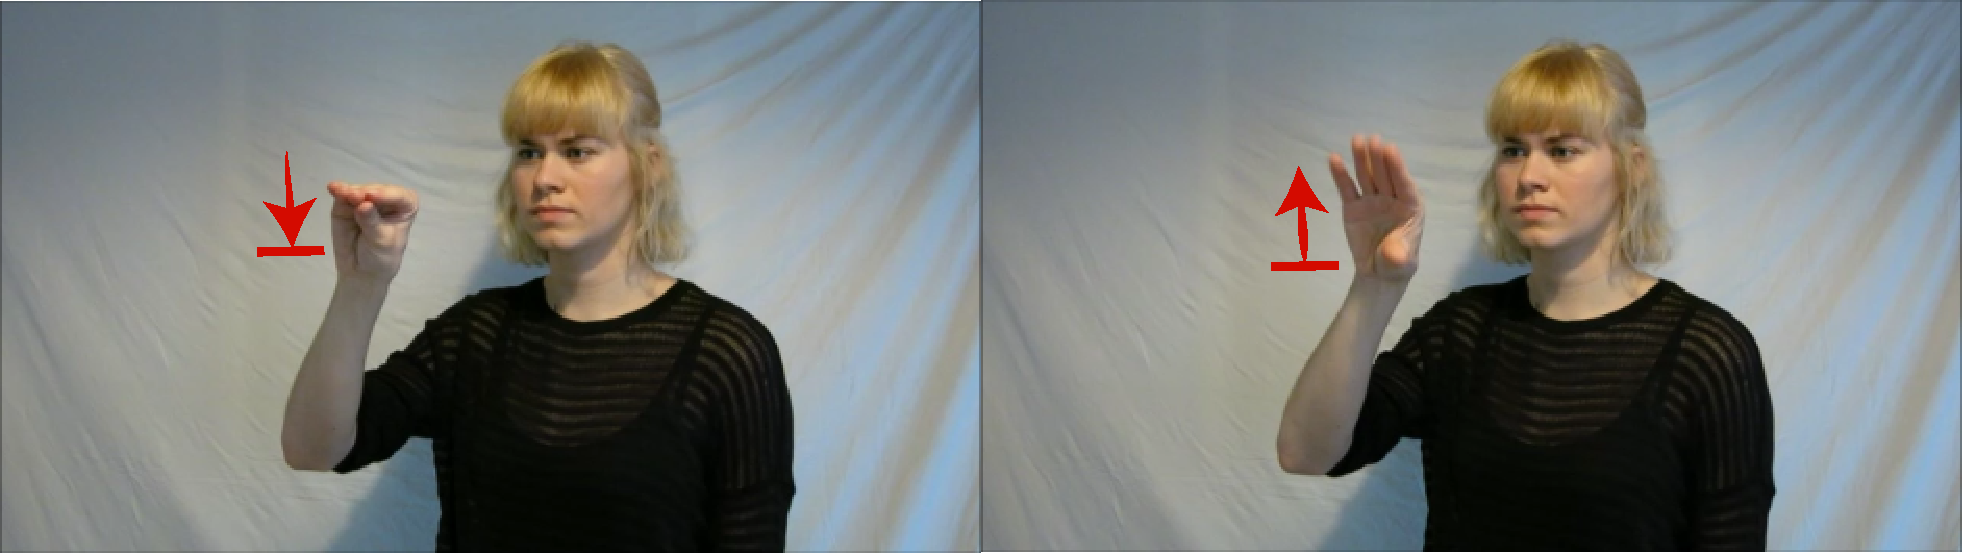
\includegraphics[resolution=300,width=0.9\textwidth]{Test1/Gestik-par/Gestik5_Pause}
	\caption{Illustration af gestik-par 5; krokodillenæb til henholdvis pause og start.}
	\label{fig:GestikPar5Pause}
\end{figure}
\noindent
%
I relation til bevægelsen i GP5 så tyder det på, at TP5 favoriserer gestik-parret, fordi bevægelsen kan udføres tæt på kroppen og der skal ikke huskes et bestemt mønster. I tillæg kommenterer TP11, at det er en lille bevægelse, faktisk den mindste bevægelse der kan laves, hvor det stadig giver mening. Af den årsag giver TP11 ydermere udtryk for, at GP5 er det eneste gestik-par, som testpersonen egentligt bryder sig om. TP7 har en anderledes tilgang til, hvorfor GP5 tildeles en førsteplads, hvilket kommer udtryk ved følgende: 
%
\begin{quotation}
	\noindent
	\textit{Altså 5'eren synes jeg var lidt sjov fordi det er sådan lidt "zip it". Jeg kunne forestille mig hvis man sådan skulle vise det frem, så kunne folk synes det var sjovt, det kan de godt huske og sådan noget.} TP7, \autoref{app:NoterValgAfGestikker}.
\noindent
\end{quotation}
%
Følgende afsnit vil omhandle forbedringsforslag fremsat af de testpersoner, som har tildelt GP5 en førsteplads.
%
\subsubsection{Forbedringsforslag til gestik-par 5}
\label{TestresultaterValgAfGestikkerForbedringGP5}
%
Af de fire testpersoner, som har valgt GP5, er der to testpersoner, som har forbedringsforslag. TP5 foreslår ingen ændringer til at pause musikken, men når musikken startes igen foreslår testpersonen, at hånden udadroterer i takt med at krokodillenæbet åbnes, hvilket resulterer i at slutpositionen er med tommelfingeren øverst. Selvom forslaget i sig selv er fint, så forventes det, at når musikken er blevet sat på pause, så skal hånden selvfølgelig ikke fastholdes i det lukkede krokodillenæb, illustreret på \autoref{fig:GestikPar5Pause}, men kunne bevæges frit. Når hånden, afslappet, frigøres fra krokodillenæbet så kan det for nogen være naturligt at lave en bevægelse, som minder om TP5's forbedringsforslag til at starte musikken, hvorfor dette forbedringsforslag afvises. Forbedringsforslaget fra TP18 kan nærmere betragtes som en selvfølge fremfor en decideret forbedring. Testpersonen foreslår nemlig, at gestikken ikke behøver at blive lavet i hovedhøjde, men bør kunne laves over alt. Grunden til at forbedringsforslaget anses som værende en selvfølge, er fordi det bør gøre sig gældende for samtlige semaforiske gestikker, at de ikke defineres ud fra en bestemt højde, men frit kan udføres.
%
\subsection{Testpersonernes begrundelse for valg af gestik-par 6}
\label{TestresultaterValgAfGestikkerBegrundelseGP6}
%
Med udgangspunkt i \autoref{fig:SamletTopTrePause} tildeles GP6 en førsteplads af to testpersoner, en andenplads af én testperson og en tredjeplads af fem testpersoner. GP6 illustreres på \autoref{fig:GestikPar6Pause}.
%
\begin{figure}[H]
	\centering
	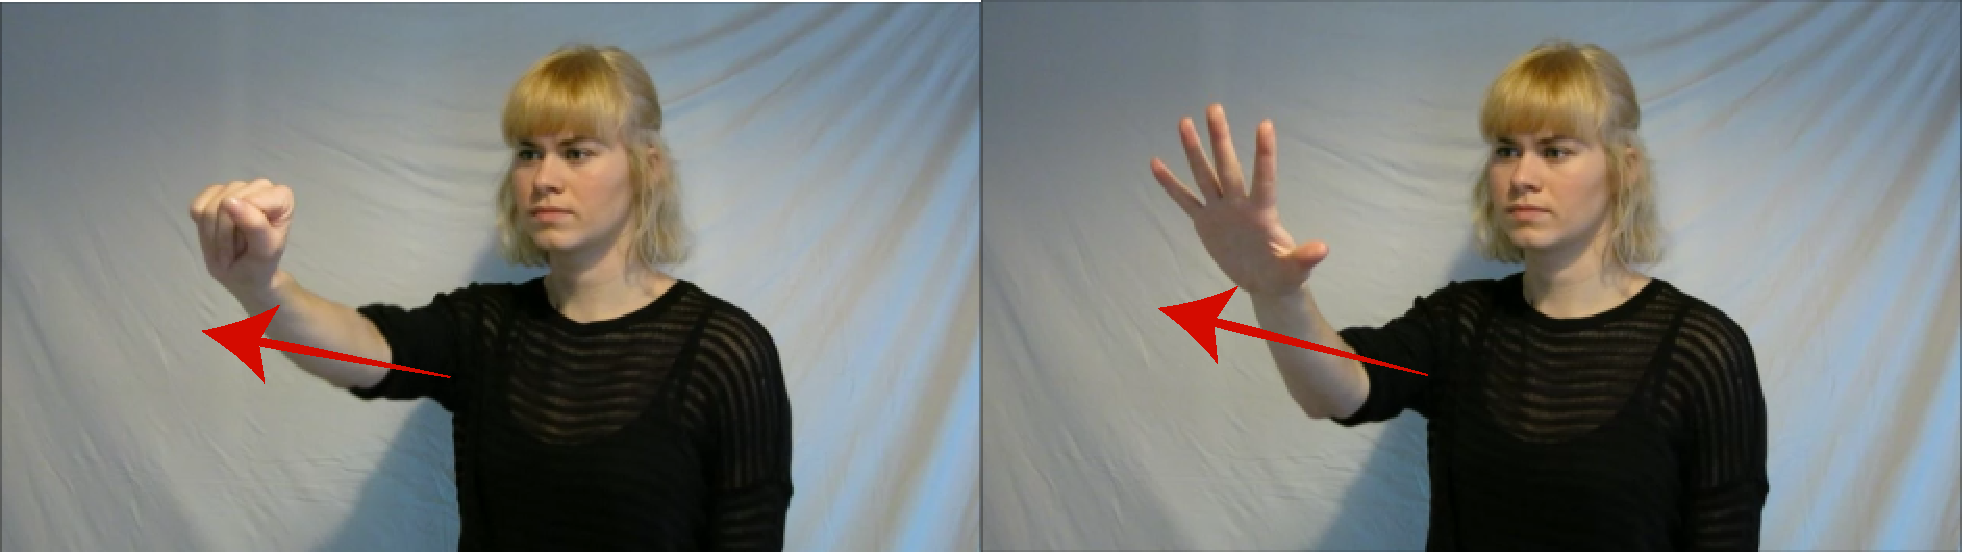
\includegraphics[resolution=300,width=0.9\textwidth]{Test1/Gestik-par/Gestik6_Pause}
	\caption{Illustration af gestik-par 6; hånden lukker sammen i en dynamisk horisontal bevægelse til pause og hånden åbner i en dynamisk horisontal bevægelse til start.}
	\label{fig:GestikPar6Pause}
\end{figure}
\noindent
%
Baseret på TP13's udsagn, kan det ikke udledes, hvorfor testpersonen foretrækker GP6, hvilket skyldes, at indtil testpersonen opfordres til at komme med et forbedringsforslag, så er det GP3, som testpersonen foretrækker. Dog kommenterer TP13, at det ikke er muligt at afgøre hvilket gestik-par, der er bedst af GP6 og GP7, fordi den eneste forskel er, hvilken retning bevægelsen foregår i. Ifølge TP14 vælges GP6, fordi det er tilpas akavet samtidig med, at det er en naturlig bevægelse i forhold til at skulle åbne og lukke lyd. Derudover pointere testpersonen, at det giver god meningen, at bevægelsen rettes mod musikanlægget. Da der kun er to testpersoner, som har rangeret GP6 på en første plads og gestik-parret sammenlagt kun indgår otte gange i testpersonernes samlede top tre rangering, samt at flere testpersoner giver udtryk for, at de åbne omkring deres anden-og tredjeplads, så vurderes det at der er belæg for at ekskludere GP6. 
%
\subsection{Testpersonernes begrundelse for valg af gestik-par 7}
\label{TestresultaterValgAfGestikkerBegrundelseGP7}
%
Med udgangspunkt i \autoref{fig:SamletTopTrePause} tildeles GP7 en førsteplads af tre testpersoner, en andenplads af tre testpersoner og en tredjeplads af fem testpersoner. GP7 illustreres på \autoref{fig:GestikPar7Pause}. De testpersoner, som har tildelt GP7 en førsteplads, begrunder det, blandt andet, ud fra en kombination af følgende egenskaber: 
%
\begin{multicols}{3}
    \begin{itemize}
        \item Simpel bevægelse
        \item Logisk bevægelse
        \item Giver mening
        \item Der er forskel 
\end{itemize}
\end{multicols}
\noindent
%
Det er begrænset hvad der kan udledes af TP8, da testpersonen til at starte med tildeler TP3 på førsteplads. Det kan dog udledes, at GP7 giver mening. Det er ligeledes svært at udlede noget konkret ud fra TP9, dog virkede det, ifølge TP9, logisk at gribe ud efter musikken for at pause den og slippe musikken fri for at starte musikken igen.
%
\begin{figure}[H]
	\centering
	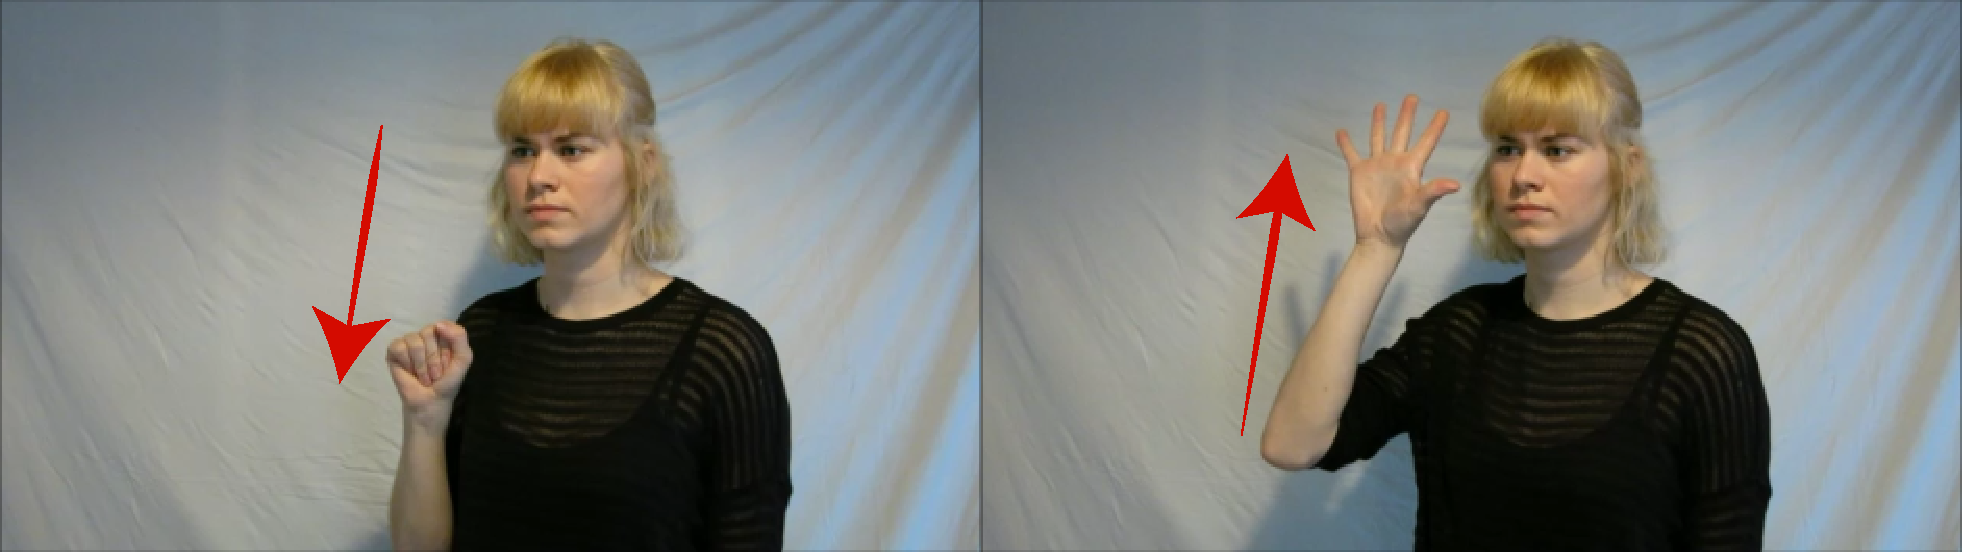
\includegraphics[resolution=300,width=0.9\textwidth]{Test1/Gestik-par/Gestik7_Pause}
	\caption{Illustration af gestik-par 7; hånden lukker sammen i en dynamisk vertikal bevægelse nedad til pause og hånden åbner i en dynamisk vertikal bevægelse opad til start.}
	\label{fig:GestikPar7Pause}
\end{figure}
\noindent
%
Da det er begrænset, hvad der kan udledes fra de tre testpersoner, som har tildelt GP7 en førsteplads og fordi GP7 trods alt sammenlagt indgår 11 gange i den samlede top tre, så vurderes det, at det er nødvendigt at inddrage de otte testpersoner, som har inkluderet GP7 andetsteds i deres top tre. De otte testpersoner, som har tildelt GP7 enten en anden- eller tredjeplads, begrunder det, blandt andet, ud fra en kombination af følgende egenskaber: 
%
\begin{multicols}{3}
    \begin{itemize}
        \item Giver mening
        \item Enkel
        \item Nem at huske
        \item Intuitiv
        \item Ikke hyppig bevægelse
\end{itemize}
\end{multicols}
\noindent
%
Baseret på begrundelserne fra de fem testpersoner, som har tildelt GP7 en tredjeplads, så skyldes det primært, at bevægelsen følger samme bevægelsesmønster, som enten den ene eller begge de gestik-par, som testpersonerne har rangeret højere. Fra \autoref{app:TopTreRangeringPauseStart} fremgår det, at hver gang en testperson tildeler GP7 en tredjeplads, så tildeles GP5 konsekvent andenpladsen. Ligende tendens går igen, når GP7 tildeles en andenplads, hvor to ud af tre testpersoner har tildelt GP5 en førsteplads. Hvis GP7 derimod indgår på en førsteplads, så er der ingen af de tre testpersoner, som inkluderer GP5, til gengæld inkluderer de GP1, GP3 og GP6.

Der er en tendens til, at testpersonerne i højere grad foretrækker enten GP1 eller GP5 over GP7. Derudover består GP5 af to forskellige bevægelser til henholdvis pause og start, som er en egenskab testpersonerne, der har inkluderet GP7, efterspørger, hvorfor det vurderes det, at der er belæg for at ekskludere GP7. 
%
\subsection{Valg af gestik-par til pause og start}
\label{TestresultaterValgAfGestikkerValgPauseStart}
%
Baseret på foregående analyse samt \autoref{app:TestresultaterPauseDaarlig}, hvor i alt fem gestik-par er ekskluderet, så står valget mellem GP1 og GP5. Fælles for de to gestik-par er, at de indgår lige mange gange i testpersonernes samlede top tre; 13 gange i alt, selvom GP1 er tildelt en førsteplads dobbelt så mange gange som GP5. Det tilstræbes at imødekomme så mange testpersoners ønske, som muligt, og flere testpersoner giver udtryk for at foretrække dels, at der er bevægelse og dels, at der er forskel på hvordan musikken sættes på pause og hvordan den startes igen, hvilket opnås i GP5.

Derudover er risikoen for at gengive GP5, ved en fejl, mindre end ved GP1. At GP1 af flere testpersoner beskrives, som værende en naturlig bevægelse, er ikke nødvendigvis et godt argument for at vælge den gestik, da stop-tegnet kan opstå i urelaterede situationer. Endvidere har seks ud af de otte testpersoner, som har tildelt GP1 en første plads, ligeledes inkluderet GP5 i deres top tre og fire ud af de seks har tildelt GP5 en andenplads. Tages alt dette i betragtning vurderes det, at der forefindes tilstrækkeligt belæg for at knytte GP5 til pause og start.

